\documentclass{beamer}
%[aspectratio=169]   \usepackage[czech]{babel}
\usepackage{apo-lecture}
\usepackage{pdfpages}
\usepackage{pdfcomment}
\usepackage{listings}
\usepackage{array,multirow}

\subtitle{Lekce 08. Výukový kit MZ\_APO (Xilinx Zynq MicroZed APO)}
\author{Pavel Píša \phantom{xxxxxxxxx} Petr Štěpán \\ \small\texttt{pisa@fel.cvut.cz}\phantom{xxxx}\small\texttt{stepan@fel.cvut.cz}}
\begin{document}

\maketitle

\section{MZ\_APO -- Xilinx Zynq MicroZed výukový kit pro B35APO}

\begin{frame}
\frametitle{Cíl dnešní přednášky}

\begin{itemize}
 \item Seznámení s komponentami/konstrukcí výukového kitu
 \item Komunikace a základní práce s kitem
 \item Princip a přístup na displej z tekutých krystalů (LCD)
 \item Barevné modely pro vykreslování
 \item Výstup písma
 \item Využití HW pro reálné aplikace
\end{itemize}
\end{frame}

\begin{frame}
\frametitle{Výukový kit MZ\_APO -- smontovaný}

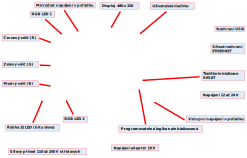
\includegraphics[width=0.98\textwidth]{mz_apo-kit-with-cover-labels.pdf}

\end{frame}

\begin{frame}
\frametitle{Výukový kit MZ\_APO -- základová deska}

\includegraphics[width=1.0\textwidth]{mz_apo-baseboard-top-labels.pdf}

\end{frame}

\begin{frame}
\frametitle{Modul MicroZed -- pohled shora}

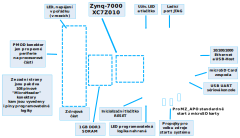
\includegraphics[width=1.0\textwidth]{microzed-board-top-labels.pdf}

\end{frame}

\begin{frame}
\frametitle{Modul MicroZed -- pohled zespodu}

MicroZed Evaluation Kit -- ADSAES-Z7MB-7Z010-G (případně AES-Z7MB-7Z010-SOM-G/REV-H cena 214\,USD)
\par
SoM -- počítač na modulu (System on Module)
\par
Čip Xilinx/AMD XC7Z010, cena okolo 90\,USD (2023)
\par
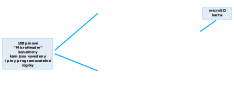
\includegraphics[width=0.90\textwidth]{microzed-board-bottom-labels.pdf}
\par
108-pinové konektory umožňují využít a propojit modul s vlastním návrhem. I přes tyto piny je možné modul napájet,
přítup k PS periferiím i pinům programovatelné logiky PL (FPGA).

\end{frame}

\begin{frame}
\frametitle{Modul MicroZed -- katalogový list}

\begin{itemize}
 \item Čip FPGA – Zynq™-7000 AP SoC (XC7Z010-CLG400-1)
 \begin{itemize}
  \item CPU: Dual ARM® Cortex™-A9 MPCore™ @ 866 MHz
  \item rychlá vnitřní statická paměť 256 kB
  \item 4400 řezů (slice) - každý řez je malý konfigurovatelný logický obvod.
    Dokáže vytvořit až 8 klopných obvodů a 4 logické funkce se 6-ti vstupy.
    Uživatel je může libovolně konfigurovat a vzájemně propojovat. (28\,K log. bloků, okolo 430\,K ekviv. log. hradel)
  \item 240\,KB (60$\times$36\,kbit) RAM a 80$\times$DSP (MAC)

 \end{itemize}
 \item Externí dynamická paměť – 1 GB DDR3
 \item Komunikace – 10/100/1000 Ethernet
 \item MicroSD karta 4 GB. V desce APO obsahuje zavaděč systému Linux pro síť Ethernet.
 \item USB Host 2.0 a USB-UART
 \item Quad-SPI Flash 128 Mb pro inicializaci při zapnutí.
 \item V APO se nepoužívá.
\end{itemize}
\end{frame}

\begin{frame}
\frametitle{Zynq™-7000 AP -- pouzdro FBGA}

\begin{columns}
\begin{column}{0.5\textwidth}
  \begin{center}
    FBGA = Fine-Pitch Ball Grid Array
    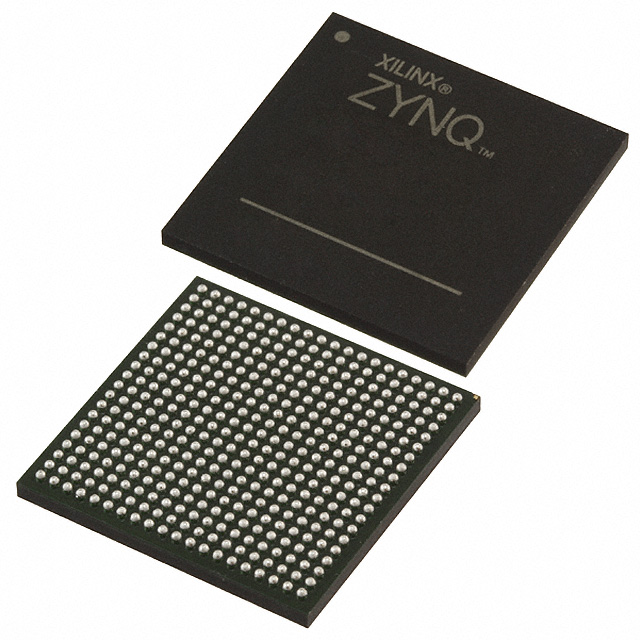
\includegraphics[width=1.0\textwidth]{fig/zynq-fbga-package.jpg}
  \end{center}
  \vfil
\end{column}
\begin{column}{0.5\textwidth}
  \begin{center}
    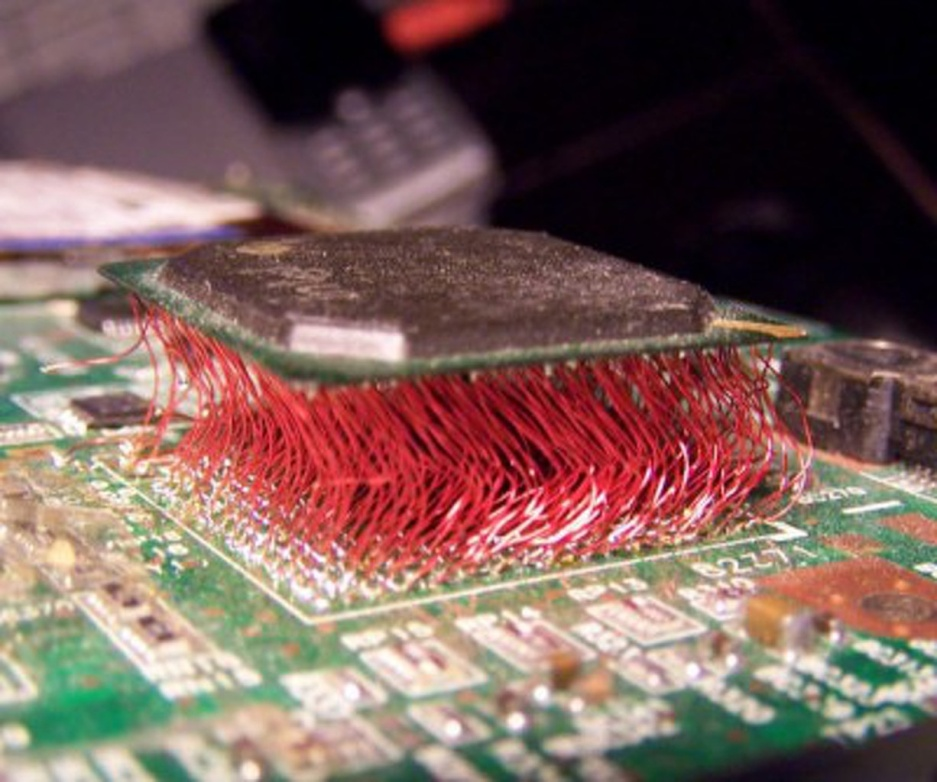
\includegraphics[width=0.55\textwidth]{fig/bga-soldering-clumsy.jpg}
    \newline
    Kuriózní pájení
    \newline
    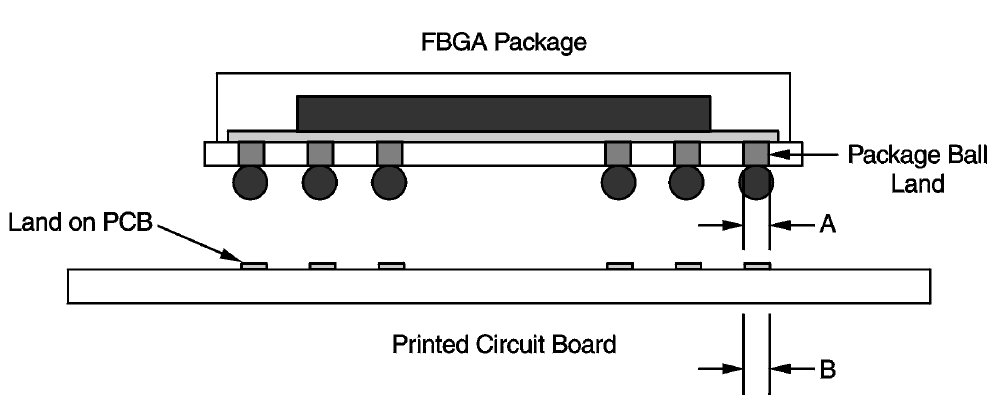
\includegraphics[width=0.8\textwidth]{fig/bga-dimensions-diagram.png}
    \newline
    Korektní pájení
    \newline
    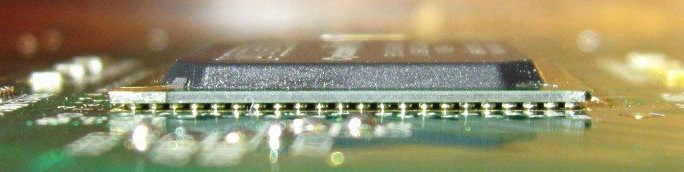
\includegraphics[width=0.8\textwidth]{fig/bga-soldering-proper.jpg}
  \end{center}
\end{column}
\end{columns}

\end{frame}

\begin{frame}
\frametitle{Xilinx Zynq-7000 -- Systém na čipu (SoC)}
  \begin{center}
    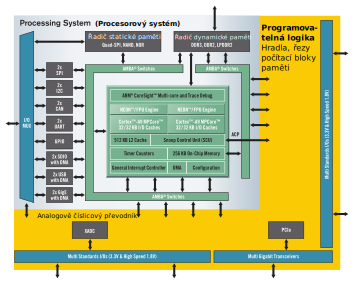
\includegraphics[width=0.73\textwidth]{xylinx-zynq-7000-block-diagram-cz.pdf}
  \end{center}
\end{frame}

\begin{frame}
\frametitle{Zvětšené jádro procesorové části}
\begin{columns}
\begin{column}{0.6\textwidth}
  \begin{center}
    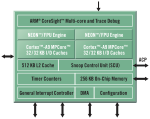
\includegraphics[width=0.95\textwidth]{xylinx-zynq-7000-block-core.pdf}
  \end{center}
  \vfil
\end{column}
\begin{column}{0.4\textwidth}
 {
 %\scriptsize
 \footnotesize
 Již jsme v APO probrali
 \begin{enumerate}
  \item Processorové jádro
  \item Aritmetiku v plovoucí řád. čárce (FPU)
  \item Skrytou pamět (Cache) instukční a datovou úroveň L1
  \item Skrytou pamět další úrovně L2
  \item Paměť na čipu (RAM)
 \end{enumerate}
 Probereme
 \begin{enumerate}
  \item Koherenci paměti -- sledovací jednotka (Snoop Control Unit)
  \item Přímý přístup k paměti (Direct Memory Access)
 \end{enumerate}
 }
\end{column}
\end{columns}
\end{frame}

\begin{frame}
\frametitle{Příklady zařízení s Cortex-A9 jádrem}

{ \scriptsize
Seznam implementací \url{https://en.wikipedia.org/wiki/ARM\_Cortex-A9\#Implementations}
}
\vspace{2mm}
\begin{columns}
\begin{column}{0.5\textwidth}
  {\scriptsize
  Asus Transformer Pad, Infinity (TF700T) \tiny \linebreak
  \url{https://en.wikipedia.org/wiki/Asus_Transformer_Pad_Infinity}
  }
  \begin{center}
    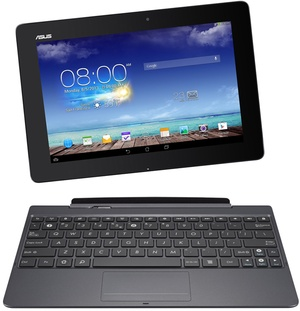
\includegraphics[width=0.7\textwidth]{fig/asus-transformer.jpg}
  \end{center}
\end{column}
\begin{column}{0.5\textwidth}
  {\scriptsize
  Apple A5 (iPhone 4S, iPad 2, iPad mini) \tiny \linebreak
  \url{http://en.wikipedia.org/wiki/Iphone_4s}
  }
  \begin{center}
    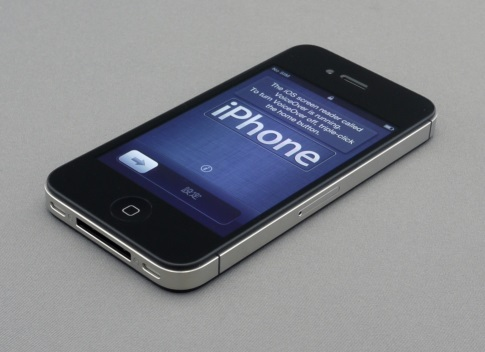
\includegraphics[width=0.5\textwidth]{fig/apple-iphone-with-a5.jpg}
  \end{center}
  {\scriptsize
  NVIDIA Tegra 2 (Motorola Xoom, Droid X2) \tiny \linebreak
  \url{http://en.wikipedia.org/wiki/Motorola_Xoom}
  }
  \begin{center}
    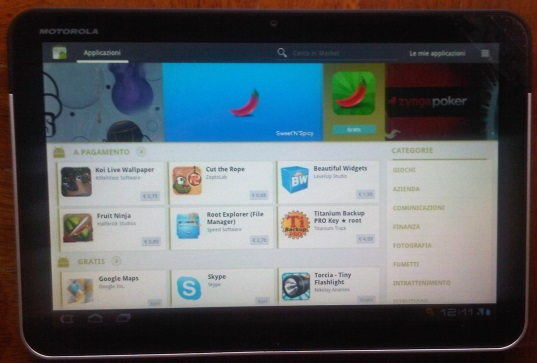
\includegraphics[width=0.4\textwidth]{fig/motorola-xoom.jpg}
  \end{center}
\end{column}
\end{columns}
\end{frame}

\begin{frame}
\frametitle{Mikroarchitektura jádra Cortex-A9}

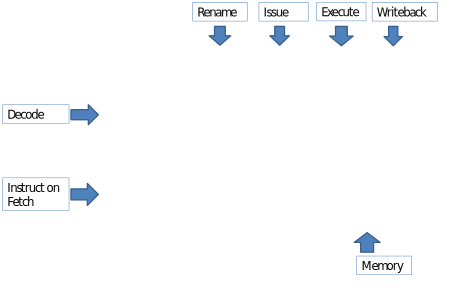
\includegraphics[width=0.95\textwidth]{cortex-a9-core-pipeline-label.pdf}

\end{frame}

\begin{frame}
\frametitle{Parematry Zynq jádra Cortex-A9}

\begin{itemize}
 \item 32 bit RISC Little Endian, 16 celočíselných registrů
 \begin{itemize}
  \item 2,5 DMIPS/MHz $\Rightarrow$ 866 MHz *2,5 DMIPS/MHz = 2165 DMIPS
  {\newline Poznámka: DMIPS je výsledkem syntetického výpočetního benchmarku Dhrystone určeného k reprezentaci celočíselného programování}
 \end{itemize}
 \item Většina celočíselných instrukcí s latencí 1 cyklus, celočíselné násobení potřebuje 4 až 5 cyklů.
 \item  Plovoucí řádová čárka prochází ALU 4 cykly pro sčítání, odečítání (FADD, FSUB), 5 cyklů pro násobení FMUL, 15 cyklů dělení FDIV (3x delší než násobení!), 17 cyklů druhé odmocniny FSQRT.
 \item Predikce větvení
 \begin{itemize}
  \item Tabulka 4\,K záznamů 2-bitových prediktorů.
 \end{itemize}
 \item Virtuální paměť se 2 úrovněmi stránkovacích tabulek
\end{itemize}

\end{frame}

\begin{frame}
\frametitle{Skrytá paměť úrovně jedna a dvě (anglicky Cache)}
\begin{itemize}
 \item 2 samostatné L1 SP pro instrukce I-cache a D-cache pro data. Vlastnosti pro obě L1:
 \begin{itemize}
  \item velikost 32\,kB
  \item 4-cestně asociativní (4-way set associative)
  \item délka bloku (řádky) 32 bajtů
  \item politika nahrazování pseudo-náhodné nebo pseudo round-robin
  \item D-Cache podporuje zpětný zápisu nebo alokace při zápisu (write-back/write-allocate policy).
 \end{itemize}
 \item L2 SP je sdílena oběma jádry Cortex-A9. Vlastnosti:
 \begin{itemize}
   \item velikost 512\,kB
   \item 8-cestně asociativní
   \item délka bloku (řádky) 32 bajtů
   \item politika výměny je pseudonáhodná,
   \item  podporuje zpětný zápis (write-back), přímý zápis (write-through) s a bez alokace
 \end{itemize}
\end{itemize}

\end{frame}

\begin{frame}
\frametitle{Stránkování pro dvě úrovně, připomenutí z před. 4. pro x86}

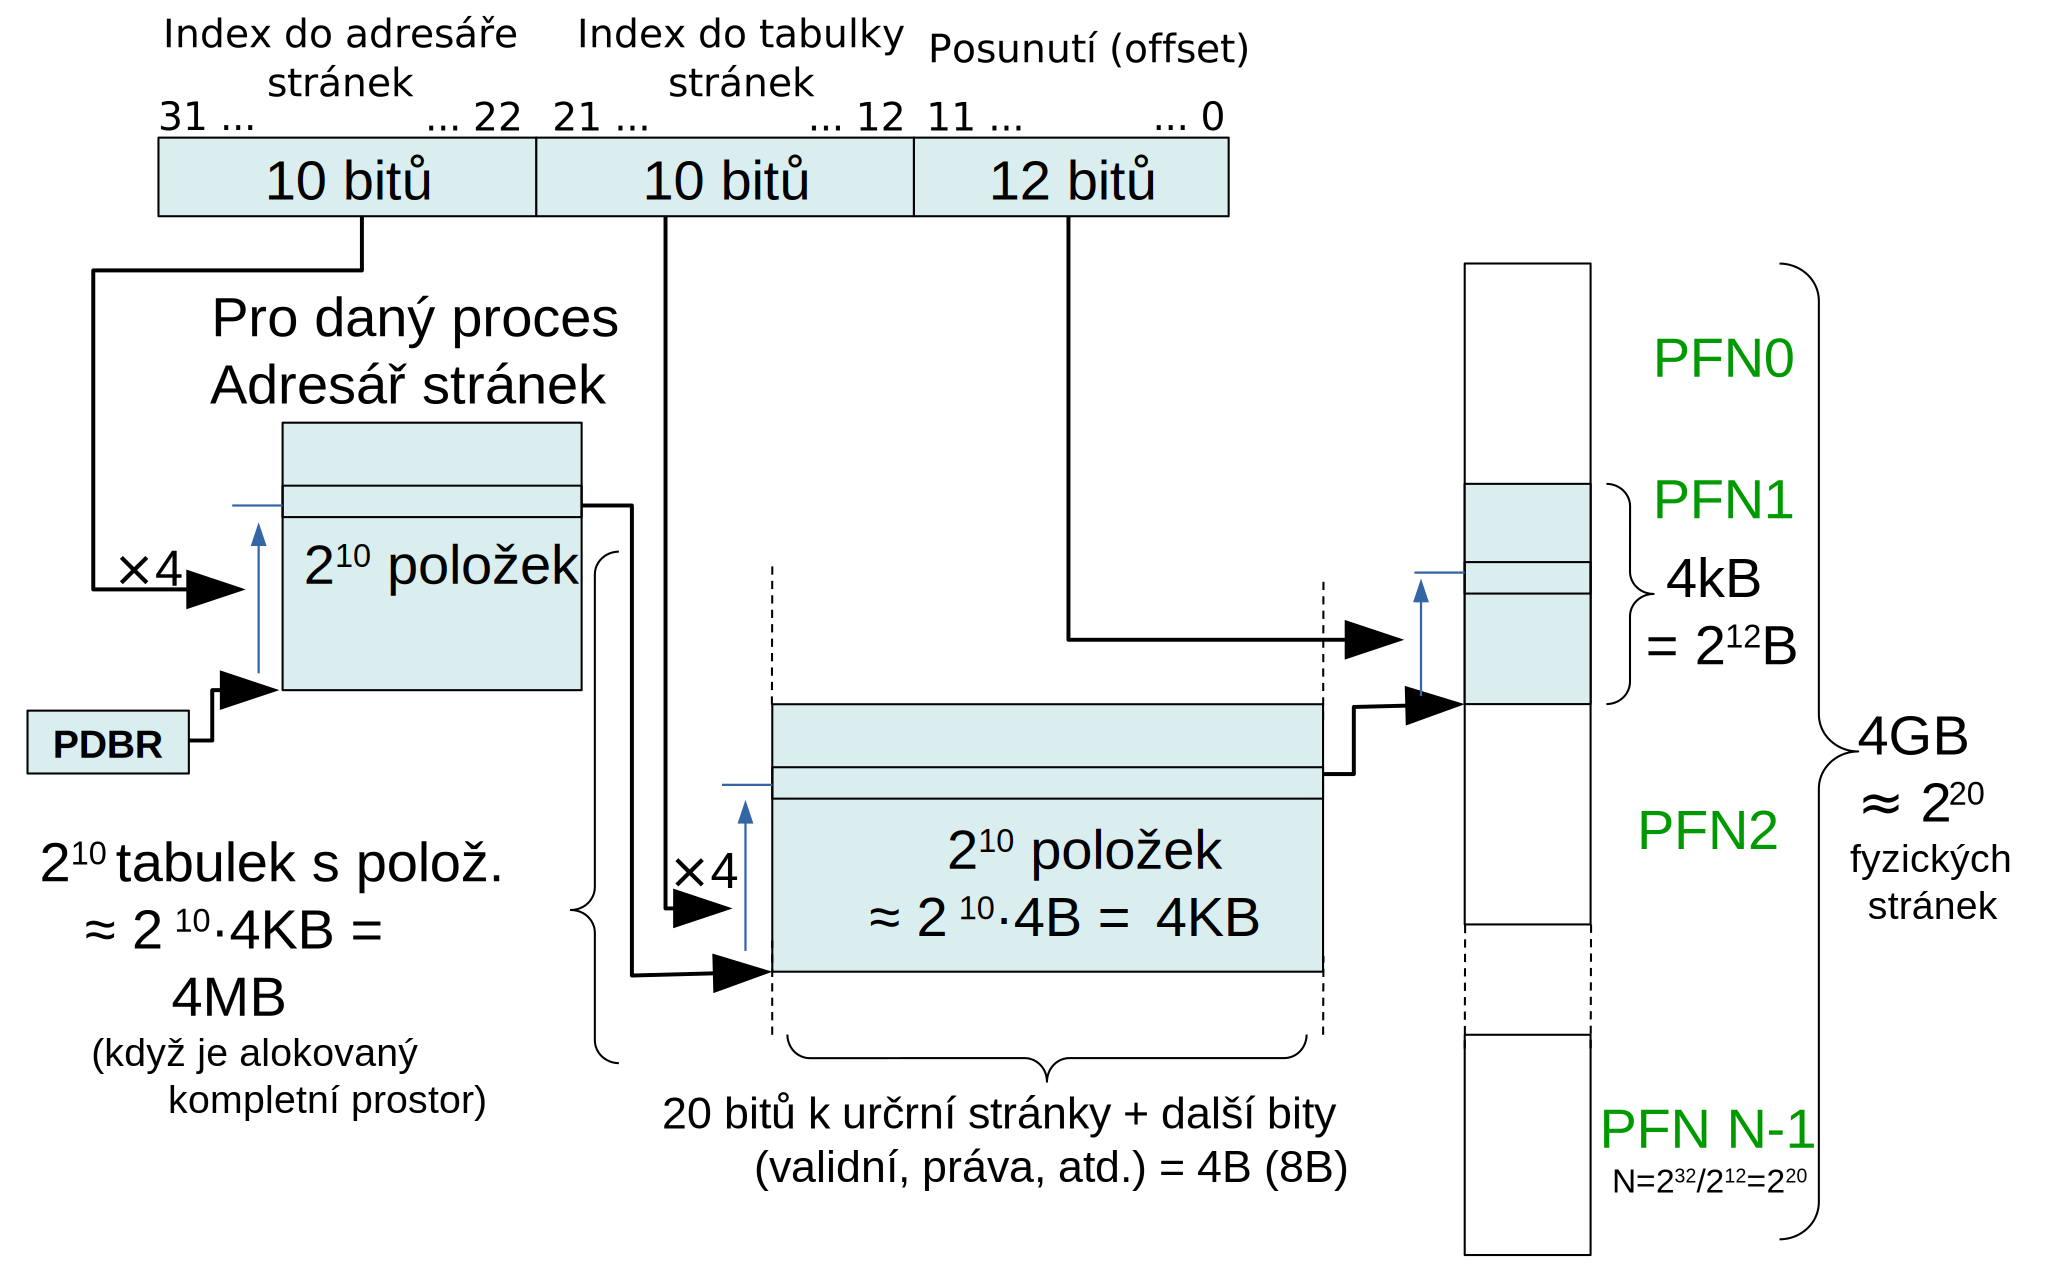
\includegraphics[width=1.0\textwidth]{paging-2-levels-cz.pdf}

\end{frame}

\begin{frame}
\frametitle{Stránkování ARM Cortex-A9 -- dvě úrovně ale nesymetrické}

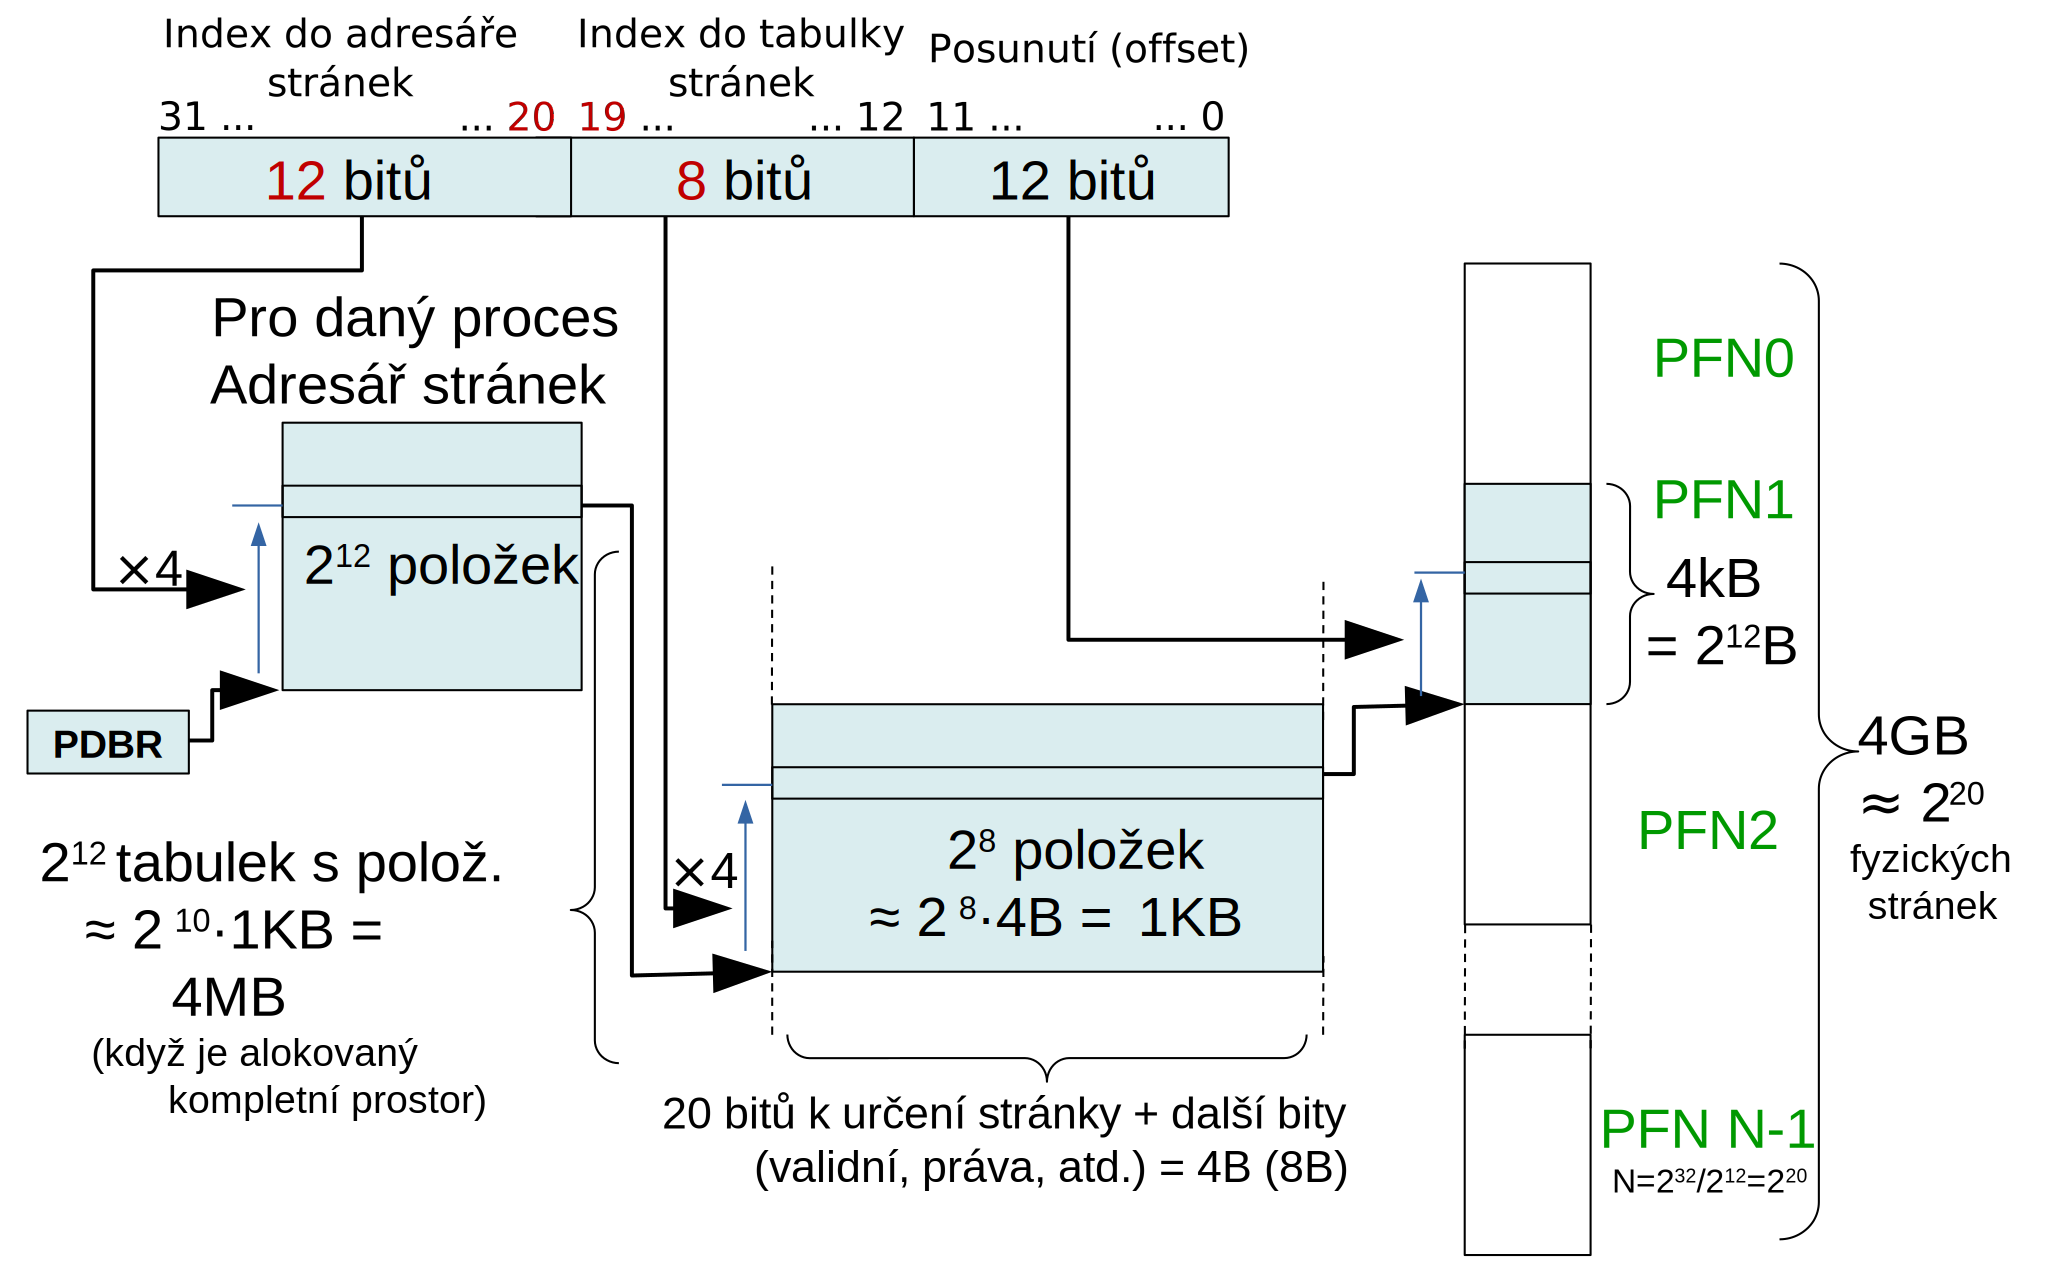
\includegraphics[width=1.0\textwidth]{paging-2-levels-cortex-a9-cz.pdf}

\end{frame}

\section{MZ\_APO -- Periferie mapované do paměťového adresního prostoru}

\begin{frame}
\frametitle{Paměťově mapované periférie, připomenutí}

\begin{itemize}
\item ARM také nemá speciální instrukce pro komunikace s perifériemi
\item pro komunikaci s perifériemi se využívá ukládání a čtení z paměti
\item Address Decoder -- rozhoduje, kam se data přesměrují
\end{itemize}
\begin{center}
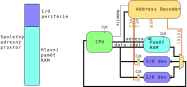
\includegraphics[width=0.88\textwidth]{address_decoder.pdf}
\end{center}
\end{frame}

\begin{frame}
\frametitle{Sběrnice AMBA AXI -- princip kanálů}

\begin{center}
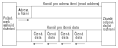
\includegraphics[width=0.55\textwidth]{amba-axi-read-concept-cz}
\end{center}

\begin{center}
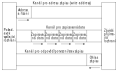
\includegraphics[width=0.55\textwidth]{amba-axi-write-concept-cz}
\end{center}

\end{frame}

\begin{frame}
\frametitle{Sběrnice AMBA AXI -- čtení}

\begin{center}
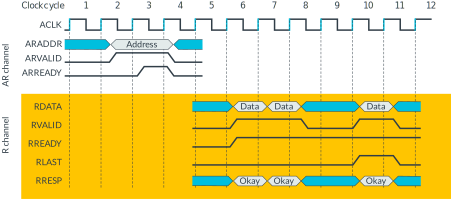
\includegraphics[width=1.0\textwidth]{amba-axi-read.pdf}
\end{center}

\begin{itemize}
\item Samostatné kanály pro adresu a data
\item Přenos proběhne vždy při souběhu xVALID a xREADY
\end{itemize}

\end{frame}

\begin{frame}
\frametitle{Sběrnice AMBA AXI -- zápis}

\begin{center}
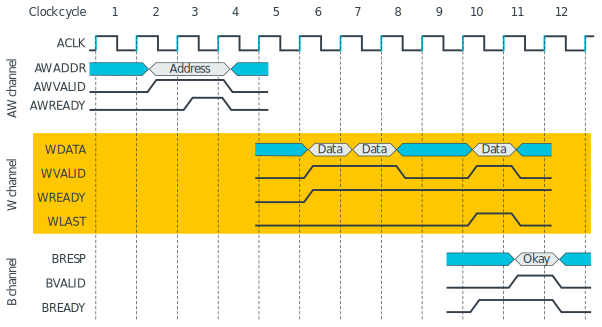
\includegraphics[width=1.0\textwidth]{amba-axi-write.pdf}
\end{center}

\end{frame}

\begin{frame}
\frametitle{Logický návrh MZ\_APO v programu Vivado}
  \begin{center}
    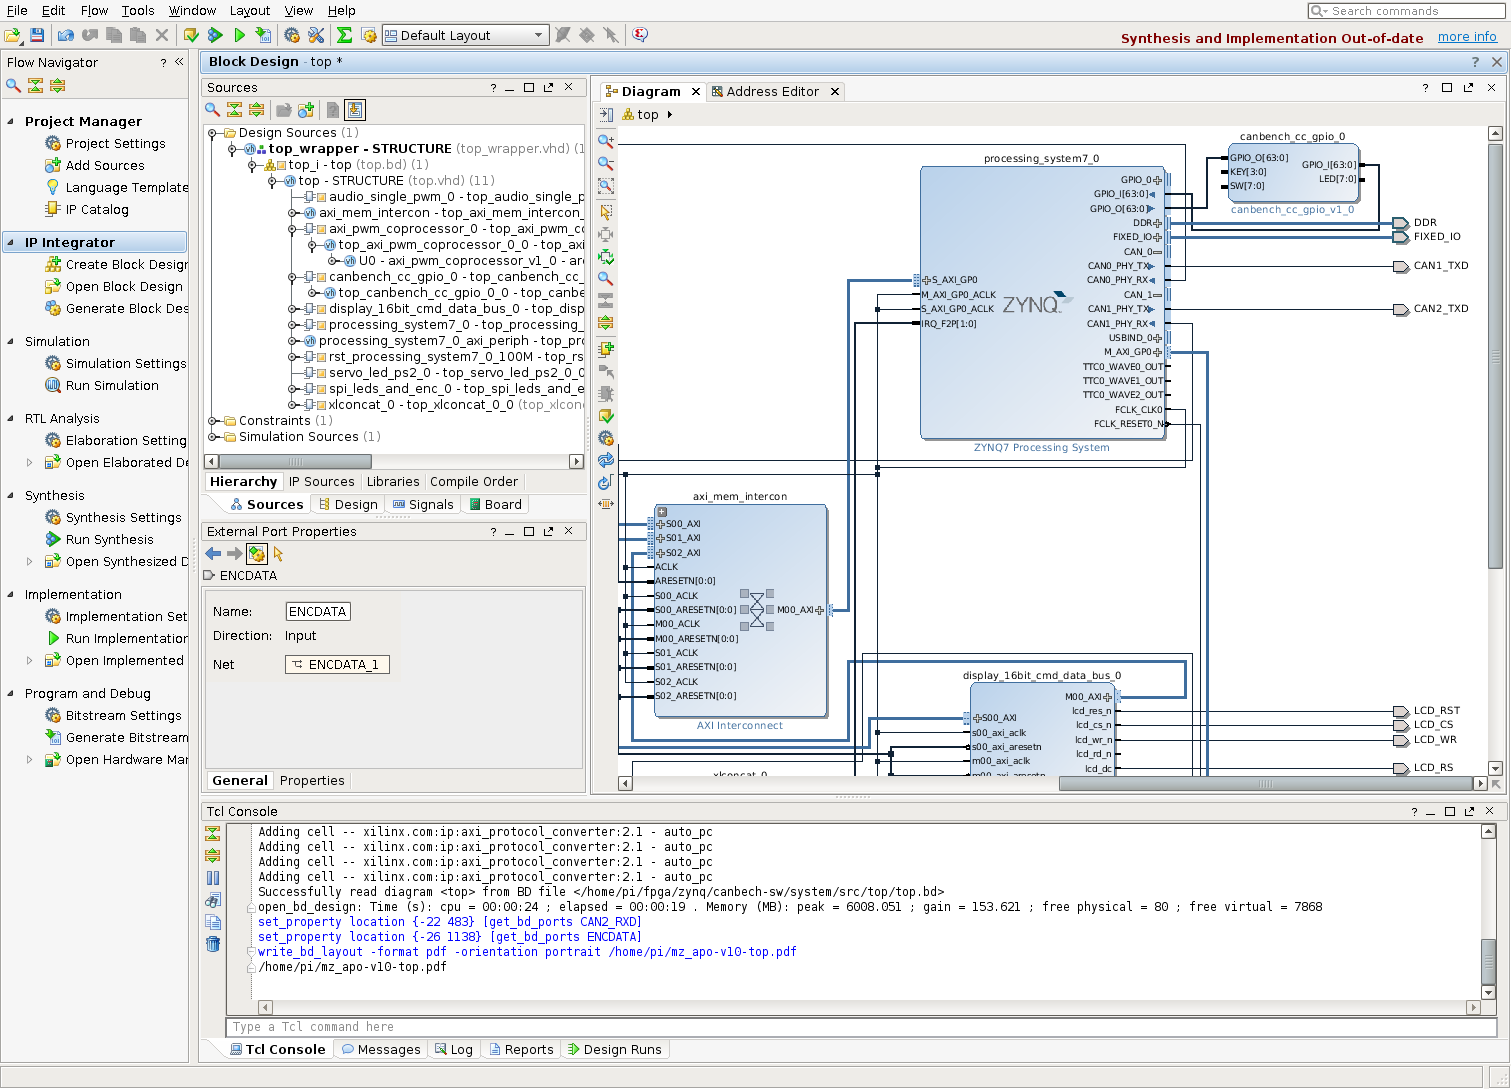
\includegraphics[width=0.8\textwidth]{fig/mz_apo-vivado-screenshot.png}
  \end{center}
\end{frame}

\begin{frame}
\frametitle{MZ\_APO -- logický návrh, propjení sběrnic a bloků}

\includegraphics[width=1.0\textwidth]{mz_apo-vivado-design.pdf}

\end{frame}

\begin{frame}
\frametitle{MZ\_APO -- Fyzické adresy výukových periferií}

\begin{tabular}{|l|l|l|l|} \hline
Bázové adresa & Délka & určení \\\hline
0x0000 0000 & 1 GB &  DRAM \\\hline
0x4000 0000 & 1 GB & port 0 sběrnice AXI do programovatelné části \\\hline
\textbf{0x43c0 0000} & 16 bytů & \textbf{APO -- LCD displej} \\\hline
0x43c2 0000 & 32 bytů & stejnosměrný motor na PMOD1 \\\hline
0x43c3 0000 & 32 bytů & stejnosměrný motor PMOD2 \\\hline
\textbf{0x43c4 0000} & 48 bytů & \textbf{APO -- periferie voličů, indikátorů} \\\hline
0x43c5 0000 & 32 bytů & 4$\times$ Servo a PS2 klávesnice \\\hline
0x43c6 0000 & 32 bytů & jednoduché audio \\\hline
0x8000 0000 & 1 GB & port 1 sběrnice AXI do programovatelné části \\\hline
0xE000 0000 &      & Reservované pro systém\\\hline
0xFFFC 0000 &      & 256 kB interní RAM \\\hline

\end{tabular} 

\end{frame}


\begin{frame}
\frametitle{Mapování rozsahu fyzického adresního prostoru do virtuálního}

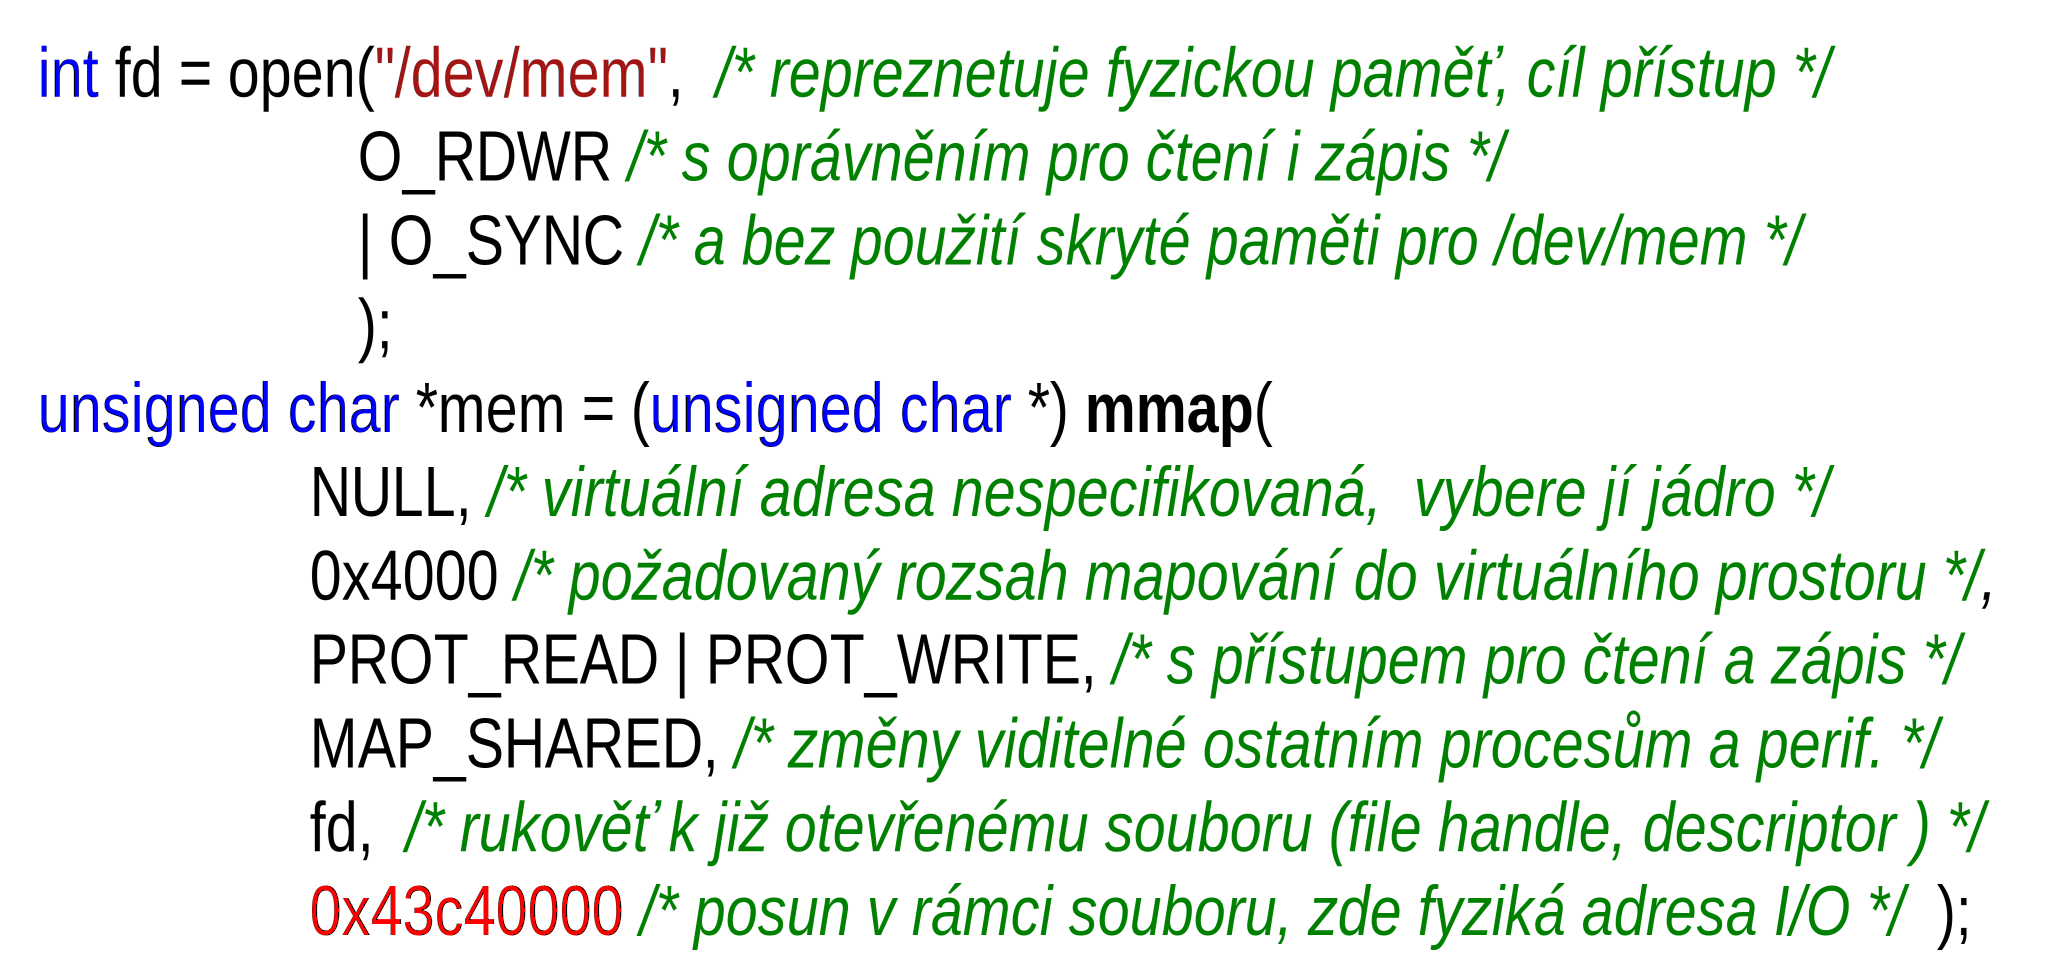
\includegraphics[width=1.0\textwidth]{mmap-phys-memory-range-cz.pdf}

\end{frame}

\begin{frame}
\frametitle{MZ\_APO -- indikátory LED a otočné voliče}

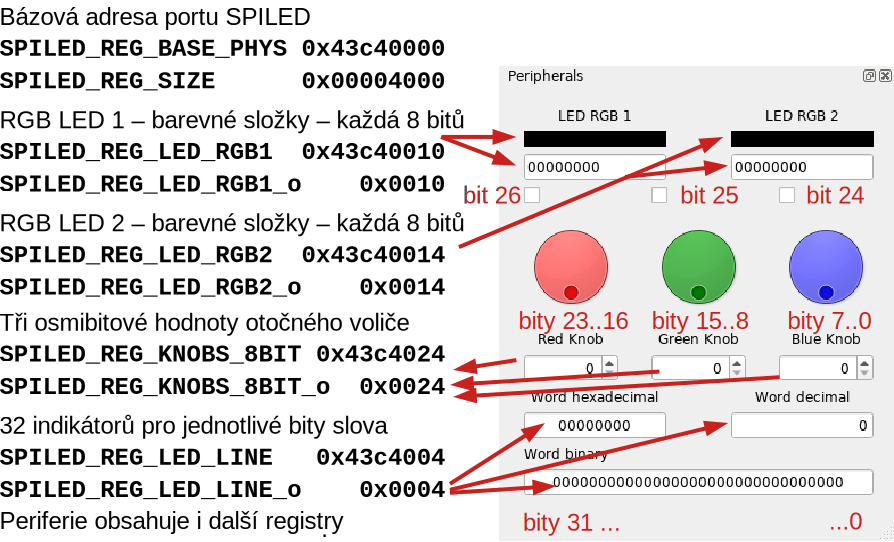
\includegraphics[width=1.0\textwidth]{mz_apo-spiled-and-knobs-cz.pdf}

\end{frame}

\begin{frame}
\frametitle{Zápis na displej na kitu MZ\_APO}

Konečný automat (FSM) přenáší data na LCD diplej generováním příslušných signálů pro řídicí čip, který periodicky obnovuje LCD TFT displej.
Pokud se objeví nový požadavek na automat dříve, než je hotový předchozí přenos, automat zbrzdí AXI sběrnici negací READY, dokud nebude moci přijmout další data/příkaz.

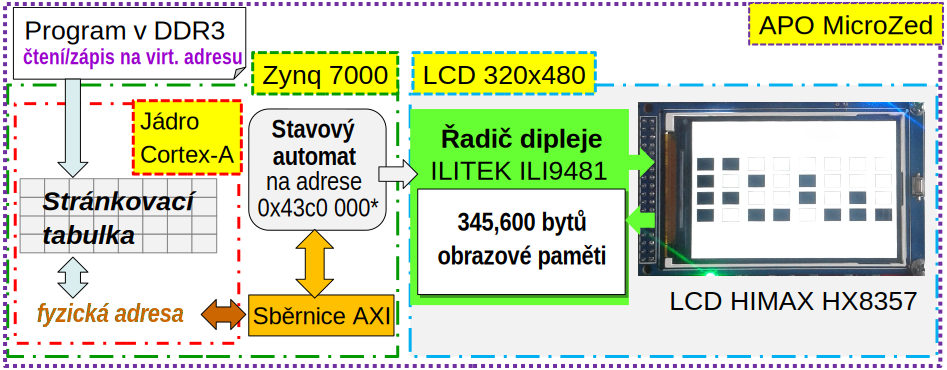
\includegraphics[width=0.9\textwidth]{mz_apo-lcd-access-cz.pdf}

\end{frame}

\begin{frame}
\frametitle{Zápis na displej na kitu MZ\_APO}

\begin{tabular}{|l|l|l|l|} \hline
Posun & \footnotesize{Datový typ} & Příkaz pro čip \\\hline
+0x0 & \footnotesize{uint16\_t} & \footnotesize{0x1 - inicializace/reset displeje, bit0 == 0 - vypnutí} \\\hline
+0x8 & \footnotesize{uint16\_t} & \footnotesize{řídicí příkaz pro kontrolér, 0x2c body od začátku} \\\hline
+0xC & \footnotesize{uint16\_t} & \footnotesize{zápis 16 bitové barvy bodu (RGB565) nebo jiných data} \\\hline
+0xC & \footnotesize{uint32\_t} & \footnotesize{zápis 2 po sobě následujících bodů: bity 15..0 a pak bity 31..0} \\\hline
\end{tabular}

\vspace{5mm}

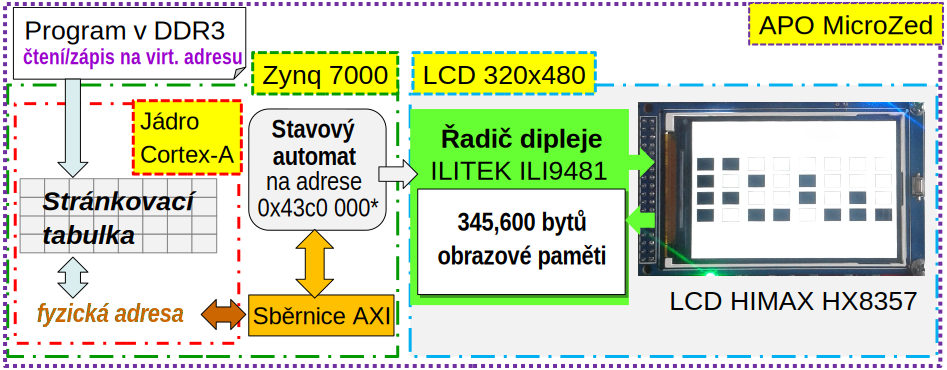
\includegraphics[width=0.9\textwidth]{mz_apo-lcd-access-cz.pdf}

\end{frame}


\end{document}

